% Fuente única de clase: Recursos/2025-11-27.pdf, páginas 1--11.
En la clase 27 caracterizamos las extensiones de Galois y describimos sus campos intermedios mediante subgrupos. Aplicamos la correspondencia a los campos finitos y a dos polinomios cúbicos; el discriminante permite distinguir sus grupos de Galois. Finalmente relacionamos la normalidad de un campo intermedio con la de su subgrupo correspondiente.

%%%%%%%%%%%%%%%%%%%%%%%%%%%%%%%%%%%%%%%%%%%%%%%%%%%%%%%%%%%%%%%%%%%%%%%%%%%%%%%
\section{Extensiones de Galois y campos fijos}
%%%%%%%%%%%%%%%%%%%%%%%%%%%%%%%%%%%%%%%%%%%%%%%%%%%%%%%%%%%%%%%%%%%%%%%%%%%%%%%
%%%%%%%%%%%%%%%%%%%%%%%%%%%%%%%%%%%%%%%%%%%%%%%%%%%%%%%%%%%%%%%%%%%%%%%%%%%%%%%
\subsection{El grado sobre un campo fijo}
%%%%%%%%%%%%%%%%%%%%%%%%%%%%%%%%%%%%%%%%%%%%%%%%%%%%%%%%%%%%%%%%%%%%%%%%%%%%%%%
% P01--P02.
El \cref{ejem:C26-cubica-real} muestra que la correspondencia de Galois no siempre es biyectiva: los campos $\mathbb Q$ y $\mathbb Q(\sqrt[3]{2})$ tienen el mismo grupo de automorfismos sobre ellos. En cambio, para extensiones finitas, cada subgrupo sí se recupera a partir de su campo fijo.

\begin{lema}\label{lema:C27-campo-fijo}
Sea $F/k$ finita y $G\leq\Aut_k(F)$. Entonces $F/F^G$ es finita, simple, normal y separable.
\end{lema}
\begin{proof}
Como $k\subseteq F^G\subseteq F$, la fórmula de la torre da $[F:F^G]\leq[F:k]<\infty$. Para $\alpha\in F$, su órbita
\[
\mathcal O_\alpha=\set{g(\alpha)\given g\in G}=\{\alpha_1,\ldots,\alpha_m\}
\]
es finita: está contenida en el conjunto de raíces en $F$ del mínimo de $\alpha$ sobre $k$. Tomamos los $\alpha_i$ distintos y definimos
\[
q_\alpha(t)=\prod_{i=1}^m(t-\alpha_i).
\]
Cada $g\in G$ permuta la órbita, de modo que su acción sobre los coeficientes satisface
\[
g(q_\alpha)(t)=\prod_{i=1}^m(t-g(\alpha_i))=q_\alpha(t).
\]
Todos sus coeficientes pertenecen, pues, a $F^G$. El mínimo de $\alpha$ sobre $F^G$ divide a $q_\alpha$, que se descompone en raíces distintas en $F$. Así cada elemento de $F$ es separable sobre $F^G$.

La extensión es finita y separable, luego el \cref{prop:C26-primitivo} permite escribir $F=F^G(\alpha)$. El polinomio $q_\alpha$ se descompone en $F$ y sus raíces generan $F$ sobre $F^G$, pues una de ellas es $\alpha$. Por tanto $F$ es su campo de descomposición y es normal por el \cref{teo:C24-normal}.
\end{proof}

\begin{prop}\label{prop:C27-artin}
Si $F/k$ es finita y $G\leq\Aut_k(F)$, entonces
\[
|G|=[F:F^G],\qquad G=\Aut_{F^G}(F).
\]
En particular, la aplicación $E\mapsto\Aut_E(F)$ de campos intermedios a subgrupos es sobreyectiva.
\end{prop}
\begin{proof}
Primero, $\Aut_k(F)$ es finito: una familia finita de generadores algebraicos determina cada automorfismo, y cada generador tiene sólo finitas imágenes posibles entre las raíces de su mínimo. En consecuencia, también $G$ es finito.

El \cref{lema:C26-correspondencia} da $G\subseteq\Aut_{F^G}(F)$. Por el lema anterior, escribamos $F=F^G(\alpha)$, con mínimo $p_\alpha$ sobre $F^G$. La normalidad y separabilidad, junto con el \cref{coro:C26-aut-normal}, dan
\[
|\Aut_{F^G}(F)|=[F:F^G]=\deg p_\alpha.
\]
El polinomio de la órbita de la prueba anterior satisface $p_\alpha\mid q_\alpha$, y su grado es a lo sumo $|G|$. Luego
\[
|G|\leq|\Aut_{F^G}(F)|=\deg p_\alpha
\leq\deg q_\alpha\leq|G|.
\]
Todas las desigualdades son igualdades, y la inclusión entre los grupos finitos es una igualdad. Así todo $G$ es la imagen del campo intermedio $F^G$.
\end{proof}

%%%%%%%%%%%%%%%%%%%%%%%%%%%%%%%%%%%%%%%%%%%%%%%%%%%%%%%%%%%%%%%%%%%%%%%%%%%%%%%
\subsection{Caracterizaciones de la condición de Galois}
%%%%%%%%%%%%%%%%%%%%%%%%%%%%%%%%%%%%%%%%%%%%%%%%%%%%%%%%%%%%%%%%%%%%%%%%%%%%%%%
% P03: ejercicio VII.4.7 reproducido íntegramente.
\begin{ejer}[Normalidad e invariancia del campo]\label{ejer:C27-normal-invariante}
Sea $F=k(\alpha)$ una extensión algebraica simple. Probar que $F/k$ es normal si y sólo si, para toda extensión algebraica $K/F$ y todo $\sigma\in\Aut_k(K)$, se cumple $\sigma(F)=F$.
\end{ejer}
\begin{sol}
Supongamos que $F/k$ es normal. Si $p$ es el mínimo de $\alpha$ sobre $k$, todas sus raíces pertenecen a $F$. Para $\sigma\in\Aut_k(K)$, $\sigma(\alpha)$ es una de esas raíces, luego
\[
\sigma(F)=k(\sigma(\alpha))\subseteq F.
\]
La restricción $\sigma:F\to\sigma(F)$ es un isomorfismo sobre $k$. Como $F/k$ es finita, la inclusión entre campos de la misma dimensión es una igualdad.

Recíprocamente, incluyamos $F$ en una clausura $\overline k$ y sea $\beta$ cualquier raíz de $p$ en ella. Existe un isomorfismo $k(\alpha)\to k(\beta)$ que fija a $k$ y envía $\alpha$ a $\beta$. Por prolongación mediante Zorn se extiende a un homomorfismo $\overline k\to\overline k$ sobre $k$. Su imagen es algebraicamente cerrada, y $\overline k$ es algebraico sobre ella; por el \cref{lema:C24-cerrado}, es un automorfismo $\sigma$.

La hipótesis aplicada a $K=\overline k$ da $\sigma(F)=F$, así que $\beta=\sigma(\alpha)\in F$. Todas las raíces de $p$ pertenecen a $F$, y $F$ es su campo de descomposición. El \cref{teo:C24-normal} prueba la normalidad.
\end{sol}

% P03--P05.
\begin{teo}\label{teo:C27-galois}
Para una extensión finita $F/k$ son equivalentes las condiciones siguientes:
\begin{enumerate}[label=(\arabic*),nosep]
\item $F$ es el campo de descomposición sobre $k$ de un polinomio separable no nulo;
\item $F/k$ es normal y separable;
\item $|\Aut_k(F)|=[F:k]$;
\item $F^{\Aut_k(F)}=k$;
\item las dos aplicaciones de la correspondencia de Galois son biyecciones inversas;
\item $F/k$ es separable y, para toda extensión algebraica $K/F$ y todo $\sigma\in\Aut_k(K)$, se tiene $\sigma(F)=F$.
\end{enumerate}
\end{teo}
\begin{proof}
$(1)\Rightarrow(2)$: el \cref{teo:C24-normal} da la normalidad. Las raíces que generan $F$ son separables sobre $k$, pues sus mínimos dividen al polinomio separable. Por la \cref{prop:C26-separable-generadores}, $F/k$ es separable.

$(2)\Rightarrow(1)$: elijamos un elemento primitivo $\alpha$. Su mínimo es separable y, por normalidad, se descompone en $F$. Como $\alpha$ genera $F$, éste es su campo de descomposición. El \cref{coro:C26-aut-normal} prueba también $(2)\Rightarrow(3)$.

$(3)\Leftrightarrow(4)$: sea $G=\Aut_k(F)$. La \cref{prop:C27-artin} y la fórmula de la torre dan
\[
|G|=[F:F^G],\qquad [F:k]=[F:F^G][F^G:k].
\]
Como los grados son finitos y positivos, $|G|=[F:k]$ equivale a $[F^G:k]=1$, es decir, a $F^G=k$. Además, $(4)\Rightarrow(2)$ por el \cref{lema:C27-campo-fijo}, aplicado a este $G$.

$(1)\Rightarrow(5)$: ya sabemos que $G=\Aut_{F^G}(F)$ para todo subgrupo. Falta probar $E=F^{\Aut_E(F)}$ para cada campo intermedio. Si $F$ es el campo de descomposición de $f\in k[t]$, también lo es de $f$ considerado en $E[t]$. Su separabilidad se conserva al ampliar coeficientes, pues no cambian las multiplicidades de las raíces. Aplicando $(1)\Rightarrow(2)\Rightarrow(3)\Rightarrow(4)$ a $F/E$, obtenemos la igualdad requerida. Ambas composiciones son la identidad.

$(5)\Rightarrow(4)$: la aplicación de campos a subgrupos envía a $k$ a $G=\Aut_k(F)$ y también envía a $F^G$ a $G$, por la \cref{prop:C27-artin}. Su inyectividad obliga a que $k=F^G$.

Por último, bajo la hipótesis de separabilidad, el elemento primitivo y el ejercicio anterior identifican normalidad con la invariancia indicada. Esto prueba $(2)\Leftrightarrow(6)$ y cierra todas las equivalencias.
\end{proof}

\begin{defi}
Una extensión finita que satisface estas condiciones es una \emph{extensión de Galois}. Su \emph{grupo de Galois} es
\[
\gal(F/k)=\Aut_k(F).
\]
\end{defi}
En lo que sigue, las extensiones de Galois son finitas. La notación $F/k$ y la inclusión $k\subseteq F$ describen la misma extensión; la barra no representa aquí un cociente de anillos.

La condición de invariancia permite visualizar la normalidad. En un campo ambiente puede haber varias imágenes conjugadas de un subcampo; cuando la extensión es de Galois, todas coinciden con el campo inicial. Los primeros dos esquemas representan estas situaciones y el tercero muestra las tres imágenes de la extensión cúbica real, con $a=\sqrt[3]{2}$ y $\omega=e^{2\pi i/3}$:

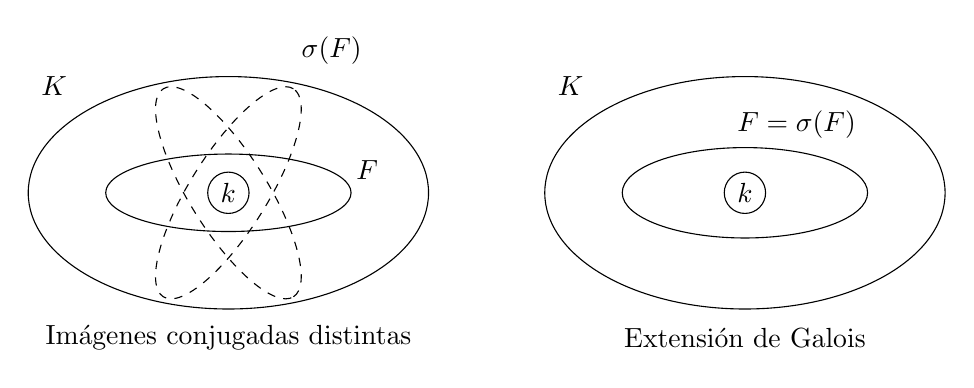
\begin{tikzpicture}[scale=.82]
\begin{scope}
\draw (0,0) ellipse (3.1 and 1.8);
\node at (-2.7,1.65) {$K$};
\draw (0,0) ellipse (1.9 and .6);
\draw[dashed,rotate=58] (0,0) ellipse (1.9 and .6);
\draw[dashed,rotate=-58] (0,0) ellipse (1.9 and .6);
\draw[fill=white] (0,0) circle (.32);
\node at (0,0) {$k$};
\node at (2.15,.35) {$F$};
\node at (1.6,2.2) {$\sigma(F)$};
\node at (0,-2.25) {Imágenes conjugadas distintas};
\end{scope}
\begin{scope}[xshift=8cm]
\draw (0,0) ellipse (3.1 and 1.8);
\node at (-2.7,1.65) {$K$};
\draw (0,0) ellipse (1.9 and .7);
\draw (0,0) circle (.32);
\node at (0,0) {$k$};
\node at (.8,1.05) {$F=\sigma(F)$};
\node at (0,-2.25) {Extensión de Galois};
\end{scope}
\end{tikzpicture}

\medskip
\begin{tikzpicture}[scale=.9]
\draw (0,0) ellipse (3.8 and 1.85);
\node at (-3.3,1.6) {$\mathbb C$};
\draw (.6,0) ellipse (2.05 and .65);
\draw[dashed,rojoDiagramaCIMAT,rotate=57] (0,0) ellipse (1.75 and .55);
\draw[dashed,rojoDiagramaCIMAT,rotate=-57] (0,0) ellipse (1.75 and .55);
\draw[fill=white] (0,0) circle (.34);
\node at (0,0) {$\mathbb Q$};
\node at (3.5,1.35) {$\mathbb Q(a)$};
\node[above=5pt] at (1.5,1.95) {$\mathbb Q(a\omega)$};
\node[below=5pt] at (1.5,-1.95) {$\mathbb Q(a\omega^2)$};
\end{tikzpicture}


%%%%%%%%%%%%%%%%%%%%%%%%%%%%%%%%%%%%%%%%%%%%%%%%%%%%%%%%%%%%%%%%%%%%%%%%%%%%%%%
\section{La correspondencia y los campos finitos}
%%%%%%%%%%%%%%%%%%%%%%%%%%%%%%%%%%%%%%%%%%%%%%%%%%%%%%%%%%%%%%%%%%%%%%%%%%%%%%%
%%%%%%%%%%%%%%%%%%%%%%%%%%%%%%%%%%%%%%%%%%%%%%%%%%%%%%%%%%%%%%%%%%%%%%%%%%%%%%%
\subsection{Grados, índices y operaciones de retículo}
%%%%%%%%%%%%%%%%%%%%%%%%%%%%%%%%%%%%%%%%%%%%%%%%%%%%%%%%%%%%%%%%%%%%%%%%%%%%%%%
% P06: comprobación remitida al ejercicio VII.6.3.
\begin{ejer}[La extensión sobre un campo intermedio]\label{ejer:C27-intermedio}
Sea $F/k$ de Galois y $k\subseteq E\subseteq F$. Probar que $F/E$ es de Galois y que
\[
[F:E]=|\Aut_E(F)|,\qquad
[E:k]=[\Aut_k(F):\Aut_E(F)].
\]
\end{ejer}
\begin{sol}
El campo $F$ es el campo de descomposición de un polinomio separable $f\in k[t]$. Sigue siendo su campo de descomposición sobre $E$, y $f$ sigue siendo separable en $E[t]$. Por el \cref{teo:C27-galois}, $F/E$ es de Galois y $[F:E]=|\Aut_E(F)|$.

La fórmula de la torre y el teorema de Lagrange dan
\[
[E:k]=\frac{[F:k]}{[F:E]}
=\frac{|\Aut_k(F)|}{|\Aut_E(F)|}
=[\Aut_k(F):\Aut_E(F)].
\]
No se afirma que $E/k$ sea de Galois. Por ejemplo, $\mathbb Q(\sqrt[3]{2})$ es intermedio en el campo de descomposición de $t^3-2$, que es de Galois sobre $\mathbb Q$, pero la extensión cúbica real no es normal.
\end{sol}

% P07.
\begin{teo}[Correspondencia de Galois]\label{teo:C27-reticulos}
Si $F/k$ es de Galois, la correspondencia es una biyección que invierte inclusiones entre el retículo de campos intermedios y el de subgrupos de $\gal(F/k)$. Si $E_i$ corresponde a $G_i$, entonces
\[
E_1E_2\ \longleftrightarrow\ G_1\cap G_2,
\qquad E_1\cap E_2\ \longleftrightarrow\ \ang{G_1,G_2}.
\]
\end{teo}
\begin{proof}
La biyección es el \cref{teo:C27-galois}, y el \cref{lema:C26-correspondencia} prueba que invierte inclusiones. Este último también da
\[
\Aut_{E_1E_2}(F)=G_1\cap G_2,
\qquad
F^{\ang{G_1,G_2}}=F^{G_1}\cap F^{G_2}=E_1\cap E_2.
\]
Las dos identidades son precisamente las correspondencias del enunciado.
\end{proof}
En la representación vertical, las aristas indican inclusiones entre los campos, y a la derecha se invierte el orden de los subgrupos:
\[
\begin{tikzcd}[column sep=huge,row sep=2em]
F\arrow[d,dash]&\{\id\}\arrow[d,dash]\\
E\arrow[d,dash]&\Aut_E(F)\arrow[d,dash]\\
k&\gal(F/k)
\end{tikzcd}
\]
En el lado de los campos, la intersección es el mayor subcampo común y el compuesto es el menor que contiene a ambos. En el lado de los grupos, esas operaciones son intersección y subgrupo generado; el teorema las intercambia.

%%%%%%%%%%%%%%%%%%%%%%%%%%%%%%%%%%%%%%%%%%%%%%%%%%%%%%%%%%%%%%%%%%%%%%%%%%%%%%%
\subsection{Frobenius y el ejemplo de sesenta y cuatro elementos}
%%%%%%%%%%%%%%%%%%%%%%%%%%%%%%%%%%%%%%%%%%%%%%%%%%%%%%%%%%%%%%%%%%%%%%%%%%%%%%%
% P07--P08.
Sea $F$ un campo finito de característica $p$. Contiene al campo primo $\mathbb F_p$. Si $d=[F:\mathbb F_p]$, una base identifica su conjunto subyacente con $\mathbb F_p^d$, luego $|F|=p^d$. Para cada $a\ne0$, Lagrange aplicado a $F^\times$ da $a^{p^d-1}=1$, y por tanto todos los elementos de $F$, incluido cero, satisfacen
\[
a^{p^d}-a=0.
\]
El polinomio $t^{p^d}-t$ tiene derivada $-1$, así que es separable. Sus $p^d$ raíces son exactamente los elementos de $F$, que es su campo de descomposición sobre $\mathbb F_p$. En particular, $F/\mathbb F_p$ es de Galois. La unicidad del campo de descomposición muestra que dos campos con $p^d$ elementos son isomorfos; se utiliza la notación $\mathbb F_{p^d}$.

También existe un campo con ese número de elementos para cada $d\geq1$. En un campo de descomposición de $t^{p^d}-t$, el conjunto de sus raíces es estable bajo suma, producto, opuestos e inversos de elementos no nulos, porque la potencia $p^d$ es un homomorfismo de campos. Las raíces forman un subcampo que contiene a $\mathbb F_p$ y genera el campo de descomposición; por ello son todo el campo. Como la derivada es $-1$, hay exactamente $p^d$ raíces distintas.

El automorfismo de Frobenius
\[
\varphi:\mathbb F_{p^d}\longrightarrow\mathbb F_{p^d},
\qquad a\longmapsto a^p
\]
fija a $\mathbb F_p$ y satisface $\varphi^d=\id$. Su orden es exactamente $d$: si $0<r<d$ y $\varphi^r=\id$, los $p^d$ elementos del campo serían raíces de $t^{p^r}-t$, cuyo grado $p^r$ es menor. Por el conteo de automorfismos de una extensión de Galois,
\[
\gal(\mathbb F_{p^d}/\mathbb F_p)=\ang{\varphi}\cong C_d.
\]

\begin{ejem}\label{ejem:C27-f64}
Para $\mathbb F_{64}/\mathbb F_2$, el grupo es $C_6$. Sus únicos subgrupos tienen órdenes $1,2,3,6$, y corresponden respectivamente a campos de tamaños $64,8,4,2$. Así los únicos campos intermedios son $\mathbb F_{64}$, $\mathbb F_8$, $\mathbb F_4$ y $\mathbb F_2$, con el siguiente par de retículos:
\begin{center}
\begin{tikzpicture}[x=1cm,y=1cm]
\node (F) at (0,2.6) {$\mathbb F_{64}$};
\node (E8) at (-1.4,1.3) {$\mathbb F_8$};
\node (E4) at (1.4,1.3) {$\mathbb F_4$};
\node (k) at (0,0) {$\mathbb F_2$};
\draw (F)--(E8)--(k)--(E4)--(F);
\draw (F)--(k);
\node (one) at (6.4,2.6) {$\{\id\}$};
\node (C2) at (4.6,1.3) {$\ang{\varphi^3}\cong C_2$};
\node (C3) at (8.2,1.3) {$\ang{\varphi^2}\cong C_3$};
\node (C6) at (6.4,0) {$\ang{\varphi}\cong C_6$};
\draw (one)--(C2)--(C6)--(C3)--(one);
\draw (one)--(C6);
\end{tikzpicture}
\end{center}

En particular,
\[
\Aut_{\mathbb F_8}(\mathbb F_{64})=\ang{\varphi^3}=\{\id,\varphi^3\},
\qquad [\mathbb F_{64}:\mathbb F_8]=2.
\]
Análogamente, $\Aut_{\mathbb F_4}(\mathbb F_{64})=\ang{\varphi^2}$ tiene orden tres. El grado de cada campo sobre $\mathbb F_2$ es el índice del subgrupo correspondiente en $C_6$.
\end{ejem}

%%%%%%%%%%%%%%%%%%%%%%%%%%%%%%%%%%%%%%%%%%%%%%%%%%%%%%%%%%%%%%%%%%%%%%%%%%%%%%%
\section{Grupos de permutaciones y discriminantes}
%%%%%%%%%%%%%%%%%%%%%%%%%%%%%%%%%%%%%%%%%%%%%%%%%%%%%%%%%%%%%%%%%%%%%%%%%%%%%%%
%%%%%%%%%%%%%%%%%%%%%%%%%%%%%%%%%%%%%%%%%%%%%%%%%%%%%%%%%%%%%%%%%%%%%%%%%%%%%%%
\subsection{La acción sobre las raíces}
%%%%%%%%%%%%%%%%%%%%%%%%%%%%%%%%%%%%%%%%%%%%%%%%%%%%%%%%%%%%%%%%%%%%%%%%%%%%%%%
% P09.
Para un polinomio separable $f\in k[t]$ con campo de descomposición $F/k$, escribimos
\[
\gal_k(f)=\gal(F/k).
\]
La elección de otro campo de descomposición produce un grupo isomorfo, mediante conjugación por un isomorfismo sobre $k$.

\begin{lema}\label{lema:C27-transitiva}
Si $f\in k[t]$ es separable e irreducible de grado $n$, su grupo de Galois actúa transitivamente sobre las raíces. Al numerarlas se identifica con un subgrupo transitivo de $S_n$.
\end{lema}
\begin{proof}
Todo automorfismo sobre $k$ permuta las raíces de $f$. La acción es fiel: si fija todas las raíces, fija el campo que generan, que es $F$.

Sean $\alpha$ y $\beta$ dos raíces. Por irreducibilidad existe un isomorfismo $k(\alpha)\to k(\beta)$ que fija a $k$ y envía $\alpha$ a $\beta$. El campo $F$ es de descomposición de $f$ sobre ambos campos. La unicidad con transporte del campo base de la \cref{prop:C24-descomposicion} prolonga ese isomorfismo a un automorfismo de $F$. Por ello cualquier raíz puede enviarse a cualquier otra.
\end{proof}

En grado tres, los únicos subgrupos transitivos, salvo conjugación, son $A_3$ y $S_3$: su orden es múltiplo de tres por órbita-estabilizador, y divide a seis por Lagrange.

En grado cuatro, las posibilidades son
\[
S_4,\qquad A_4,\qquad D_8,\qquad C_2\times C_2,\qquad C_4.
\]
Para justificar la lista, el orden de un subgrupo transitivo de $S_4$ es múltiplo de cuatro y divide a $24$, luego es $4,8,12$ o $24$. Un grupo de orden cuatro es $C_4$ o $C_2\times C_2$, y su acción transitiva sobre cuatro puntos es regular: los estabilizadores son triviales. Los subgrupos de orden ocho son los de Sylow de $S_4$, conjugados al grupo de simetrías de un cuadrado, $D_8$. Un subgrupo de orden doce tiene índice dos y es el núcleo de un homomorfismo sobreyectivo $S_4\to C_2$. Todas las transposiciones son conjugadas y generan $S_4$, de modo que todas se envían al elemento no trivial; el homomorfismo es el signo y su núcleo es $A_4$. El caso de orden $24$ es $S_4$.

%%%%%%%%%%%%%%%%%%%%%%%%%%%%%%%%%%%%%%%%%%%%%%%%%%%%%%%%%%%%%%%%%%%%%%%%%%%%%%%
\subsection{El discriminante y el grupo alternante}
%%%%%%%%%%%%%%%%%%%%%%%%%%%%%%%%%%%%%%%%%%%%%%%%%%%%%%%%%%%%%%%%%%%%%%%%%%%%%%%
% P09--P10.
Sea $f\in k[t]$ mónico y separable, con raíces $\alpha_1,\ldots,\alpha_n$ en su campo de descomposición. Definimos
\[
\Delta=\prod_{1\leq i<j\leq n}(\alpha_i-\alpha_j),
\qquad D=\Delta^2.
\]
El elemento $D$ es el \emph{discriminante} de $f$. Como las raíces son distintas, $\Delta\ne0$. Una transposición de dos raíces cambia el signo de $\Delta$; por composición, cualquier permutación $\pi$ satisface $\pi(\Delta)=\operatorname{sgn}(\pi)\Delta$. Por tanto toda permutación fija a $D$, y la correspondencia de Galois da $D\in k$. Para estudiar un polinomio no mónico mediante este criterio, podemos dividirlo por su coeficiente principal: el asociado mónico tiene las mismas raíces y el mismo grupo de Galois.

\begin{lema}\label{lema:C27-discriminante}
Supongamos que $\operatorname{char}k\ne2$. Para un polinomio mónico separable $f$ de grado $n$, se tiene $\gal_k(f)\subseteq A_n$ si y sólo si su discriminante es un cuadrado en $k$.
\end{lema}
\begin{proof}
Como $\Delta\ne0$ y $-\Delta\ne\Delta$, el grupo fija a $\Delta$ exactamente cuando sus permutaciones son pares. Por la condición de campo fijo, esto equivale a $\Delta\in k$, que hace de $D=\Delta^2$ un cuadrado del campo base.

Si $D=d^2$ para algún $d\in k$, entonces $\Delta^2=d^2$, de donde $(\Delta-d)(\Delta+d)=0$. Como estamos en un campo, $\Delta=d$ o $\Delta=-d$. Así $\Delta\in k$ y todas las permutaciones del grupo son pares.
\end{proof}

Para una cúbica mónica
\[
f(t)=t^3+at^2+bt+c,
\]
la expansión del producto de diferencias, usando las relaciones entre raíces y coeficientes, da
\[
D=a^2b^2-4a^3c-4b^3+18abc-27c^2.
\]
Si además la característica es distinta de tres, conviene eliminar el término cuadrático:
\[
f\left(t-\frac a3\right)=t^3+pt+q,
\qquad p=b-\frac{a^2}{3},\qquad q=c-\frac{ab}{3}+\frac{2a^3}{27}.
\]
Trasladar todas las raíces por la misma cantidad no cambia sus diferencias, por lo que no cambia $D$. Para $g(t)=t^3+pt+q$, la fórmula se reduce a
\[
D=-4p^3-27q^2.
\]
Podemos comprobarla directamente. Si $r,s,u$ son las raíces, entonces
\[
r+s+u=0,\quad rs+ru+su=p,\quad rsu=-q,
\]
de donde $r^2+s^2+u^2=-2p$ y $r^2s^2+r^2u^2+s^2u^2=p^2$. Además,
\[
\begin{aligned}
-D&=g'(r)g'(s)g'(u)\\
&=(3r^2+p)(3s^2+p)(3u^2+p)\\
&=27q^2+9p\,p^2+3p^2(-2p)+p^3
=27q^2+4p^3.
\end{aligned}
\]
La primera igualdad sigue de $g'(r)=(r-s)(r-u)$ y las dos identidades análogas. Sustituir $p$ y $q$ recupera la fórmula general. Esta última es una identidad con coeficientes enteros, por lo que también vale en característica tres, aunque allí no se puede efectuar el cambio $t\mapsto t-a/3$.

Si la cúbica es irreducible y separable y la característica es distinta de dos, su grupo es $A_3$ cuando $D$ es un cuadrado, y $S_3$ cuando no lo es: ésas son las dos posibilidades transitivas del grado tres.

%%%%%%%%%%%%%%%%%%%%%%%%%%%%%%%%%%%%%%%%%%%%%%%%%%%%%%%%%%%%%%%%%%%%%%%%%%%%%%%
\subsection{Dos ejemplos cúbicos}
%%%%%%%%%%%%%%%%%%%%%%%%%%%%%%%%%%%%%%%%%%%%%%%%%%%%%%%%%%%%%%%%%%%%%%%%%%%%%%%
% P10--P11.
\begin{ejem}[El campo de descomposición de $t^3-2$]\label{ejem:C27-s3}
El polinomio $t^3-2$ es irreducible sobre $\mathbb Q$ por Eisenstein con $2$ y es separable por característica cero. Su discriminante es
\[
D=-27(-2)^2=-108,
\]
que no es un cuadrado racional. Por tanto $\gal_{\mathbb Q}(t^3-2)\cong S_3$.

Pongamos $a=\sqrt[3]{2}\in\mathbb R$ y $\omega=e^{2\pi i/3}$. El campo de descomposición es
\[
L=\mathbb Q(a,a\omega,a\omega^2)=\mathbb Q(a,\omega).
\]
La primera igualdad con la segunda se debe a que $\omega=(a\omega)/a$ y a que las tres raíces pertenecen a $\mathbb Q(a,\omega)$. Como $\mathbb Q(a)\subseteq\mathbb R$ y $\omega$ no es real, su mínimo sobre ese campo es $t^2+t+1$. Así $[L:\mathbb Q]=2\cdot3=6$, de acuerdo con el orden de $S_3$.

Podemos elegir los automorfismos
\[
\begin{array}{c|cc}
&a&\omega\\\hline
\sigma&a\omega&\omega\\
\tau&a&\omega^2
\end{array}
\]
Como $[L:\mathbb Q(\omega)]=3$, el mínimo de $a$ sobre $\mathbb Q(\omega)$ es $t^3-2$. La existencia de $\sigma$ se obtiene extendiendo el isomorfismo que envía $a$ a $a\omega$ sobre esa base, mediante la unicidad de campos de descomposición. El automorfismo $\tau$ es la conjugación compleja. Se cumple
\[
\sigma^3=\tau^2=\id,\qquad \tau\sigma\tau=\sigma^{-1},
\qquad \gal(L/\mathbb Q)=\ang{\sigma,\tau}\cong S_3.
\]
La relación de conjugación se comprueba en los generadores $a$ y $\omega$; los seis elementos $\sigma^i$ y $\tau\sigma^i$, $0\leq i<3$, son distintos por sus imágenes de esos generadores.

Los dos retículos son
\begin{center}
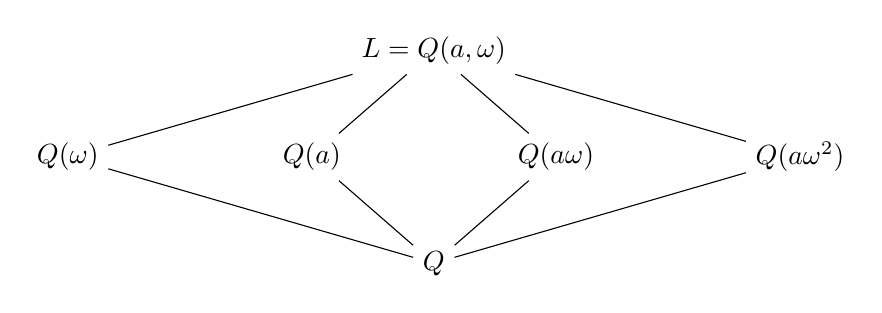
\begin{tikzpicture}[x=1cm,y=1cm]
\node (L) at (4.65,2.7) {$L=\mathbb Q(a,\omega)$};
\node (E0) at (0,1.35) {$\mathbb Q(\omega)$};
\node (E1) at (3.1,1.35) {$\mathbb Q(a)$};
\node (E2) at (6.2,1.35) {$\mathbb Q(a\omega)$};
\node (E3) at (9.3,1.35) {$\mathbb Q(a\omega^2)$};
\node (Q) at (4.65,0) {$\mathbb Q$};
\foreach \j in {0,1,2,3}{\draw (L)--(E\j)--(Q);}
\end{tikzpicture}

\medskip
\begin{tikzpicture}[x=1cm,y=1cm]
\node (one) at (4.65,2.7) {$\{\id\}$};
\node (H0) at (0,1.35) {$\ang{\sigma}=A_3$};
\node (H1) at (3.1,1.35) {$\ang{\tau}$};
\node (H2) at (6.2,1.35) {$\ang{\tau\sigma}$};
\node (H3) at (9.3,1.35) {$\ang{\tau\sigma^2}$};
\node (G) at (4.65,0) {$\ang{\sigma,\tau}=S_3$};
\foreach \j in {0,1,2,3}{\draw (one)--(H\j)--(G);}
\end{tikzpicture}
\end{center}

El campo $\mathbb Q(\omega)$ corresponde a $\ang{\sigma}=A_3$; su grado sobre $\mathbb Q$ es dos y $[L:\mathbb Q(\omega)]=3$. Los tres campos cúbicos corresponden a los tres subgrupos de orden dos, que tienen índice tres. En concreto,
\[
\begin{aligned}
L^{\ang{\tau}}&=\mathbb Q(a),\\
L^{\ang{\tau\sigma}}&=\mathbb Q(a\omega),\\
L^{\ang{\tau\sigma^2}}&=\mathbb Q(a\omega^2).
\end{aligned}
\]
Con la composición de funciones, el subgrupo indicado fija al generador correspondiente. El campo fijo y el campo de la derecha tienen grado tres sobre $\mathbb Q$, por lo que coinciden.

La conjugación por $\sigma$ permuta los tres subgrupos de orden dos y sus campos fijos. Por ejemplo, $\tau$ fija a $a$, pero $\sigma$ envía $\mathbb Q(a)$ a $\mathbb Q(a\omega)\ne\mathbb Q(a)$. Por tanto $\ang{\tau}$ no es normal en $S_3$, y $\mathbb Q(a)/\mathbb Q$ no es normal. En cambio, las extensiones de $L$ sobre todos sus campos intermedios sí son de Galois.
\end{ejem}

\begin{ejem}[Un grupo cíclico de orden tres]
El polinomio $f(t)=t^3-3t+1$ no tiene raíces racionales: las únicas posibilidades son $1$ y $-1$, y ninguna lo anula. Por ser cúbico, es irreducible sobre $\mathbb Q$. Es separable y su discriminante es
\[
D=-4(-3)^3-27=108-27=81=9^2.
\]
Así $\gal_{\mathbb Q}(f)=A_3\cong C_3$. Su campo de descomposición tiene grado tres sobre $\mathbb Q$; en particular, queda generado por cualquiera de sus raíces, porque cada una tiene grado tres y pertenece a él.
\end{ejem}

%%%%%%%%%%%%%%%%%%%%%%%%%%%%%%%%%%%%%%%%%%%%%%%%%%%%%%%%%%%%%%%%%%%%%%%%%%%%%%%
\section{Campos intermedios normales y grupos cociente}
%%%%%%%%%%%%%%%%%%%%%%%%%%%%%%%%%%%%%%%%%%%%%%%%%%%%%%%%%%%%%%%%%%%%%%%%%%%%%%%
% P11: enunciado VII.6.15; se desarrolla la prueba por conjugación/restricción.
\begin{teo}\label{teo:C27-cociente}
Sea $F/k$ de Galois y sea $k\subseteq E\subseteq F$. Entonces $E/k$ es de Galois si y sólo si $\Aut_E(F)$ es normal en $\Aut_k(F)$. En ese caso, la restricción induce un isomorfismo
\[
\gal(E/k)\cong\gal(F/k)/\Aut_E(F).
\]
\end{teo}
\begin{proof}
Sean $G=\gal(F/k)$ y $H=\Aut_E(F)$. Como $E=F^H$, para $g\in G$ tenemos
\[
g(F^H)=F^{gHg^{-1}}.
\]
En efecto, si $x$ está fijo por $H$ y $h\in H$, entonces $(ghg^{-1})(g(x))=g(h(x))=g(x)$. La inclusión inversa se obtiene aplicando el mismo argumento a $g^{-1}$.

Si $E/k$ es de Galois, es normal y el \cref{ejer:C27-normal-invariante} da $g(E)=E$ para todo $g\in G$. La identidad anterior y la inyectividad de la correspondencia implican $gHg^{-1}=H$, luego $H$ es normal.

Recíprocamente, si $H$ es normal, la identidad da $g(E)=E$ para todo $g\in G$. Todo elemento de $E$ es separable sobre $k$, pues lo es en $F$. Para probar normalidad, elijamos $\alpha\in E$ y cualquier raíz $\beta\in\overline k$ de su mínimo sobre $k$. La normalidad de $F/k$ garantiza $\beta\in F$. El isomorfismo $k(\alpha)\to k(\beta)$ se prolonga a un automorfismo $g$ de $F$, usando que $F$ es campo de descomposición de un polinomio de $k[t]$ sobre ambas bases. Entonces $\beta=g(\alpha)\in g(E)=E$. El mínimo se descompone en $E$, de modo que $E/k$ es normal y, junto con la separabilidad, es de Galois.

En estas condiciones, la restricción es un homomorfismo de grupos
\[
\rho:G\longrightarrow\gal(E/k),\qquad g\longmapsto\restr{g}{E},
\]
con núcleo $H$. Es sobreyectiva: para $u\in\gal(E/k)$, tomemos un polinomio separable de $k[t]$ cuyo campo de descomposición sea $F$. Considerado en $E[t]$, $u$ no cambia sus coeficientes y $F$ es su campo de descomposición sobre $E$. La unicidad con transporte de la base prolonga $u$ a un automorfismo de $F$ sobre $k$. El primer teorema de isomorfismo da $G/H\cong\gal(E/k)$.
\end{proof}

Para el ejemplo cúbico anterior, $A_3$ es normal en $S_3$ y
\[
\gal(\mathbb Q(\omega)/\mathbb Q)\cong S_3/A_3\cong C_2.
\]
Los tres subgrupos de orden dos no son normales; sus campos cúbicos correspondientes son separables sobre $\mathbb Q$, pero no son extensiones de Galois.

\begin{obs}[Referencias de lectura]
En \citet[cap.~VII]{aluffi2009}, los campos fijos y las extensiones de Galois se estudian en 6.5--6/9--11; los retículos y grupos cociente, en 6.12/15; la acción en raíces y los discriminantes, en 7.17--19. Los ejercicios resueltos corresponden a VII.4.7 y VII.6.3.
\end{obs}
